Bivariate choropleth maps follow the same concept as univariate choropleth maps (see chapter \ref{s:choropleth} on page \pageref{s:choropleth} for more information), except they show two phenomenons at once. Therefore two datasets need to be combined to show how much of the first variable and the second variable exist in each enumeration unit. The main concept and design goals aswell as data standardization and classification still apply to the multivariate version. The only adaption pertains to the color scale. Figure \ref{fig:bi-scale} on page \pageref{fig:bi-scale} shows two possible color scales. The main difference between sequential and diverging color scales are already explained in detail and therefore using either a sequential (see figure \ref{fig:bi-seq} on page \pageref{fig:bi-seq}) or diverging (see figure \ref{fig:bi-div} on page \pageref{fig:bi-div}) color scale matrix should be clear.


\begin{figure}[!htb]
  \captionsetup[subfigure]{justification=centering}
  \centering
  \begin{subfigure}[b]{0.4\textwidth}
    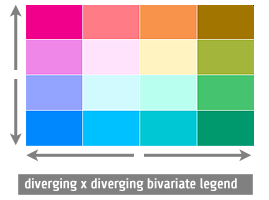
\includegraphics[width=\textwidth]{images/choropleth/divxdiv.png}
    \caption{Diverging x diverging bivariate color scale.}
    \label{fig:bi-div}
  \end{subfigure}
  \hfill
  \begin{subfigure}[b]{0.4\textwidth}
    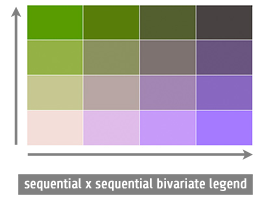
\includegraphics[width=\textwidth]{images/choropleth/seqxseq.png}
    \caption{Sequential x sequential bivariate color scale.}
    \label{fig:bi-seq}
  \end{subfigure}
  \caption[
    Bivariate color scale for choropleth maps, Urldate: 07.2016 \newline
    \small\texttt{\url{https://axismaps.github.io/thematic-cartography/images/seqxseq.png}} \newline
    \small\texttt{\url{https://axismaps.github.io/thematic-cartography/images/divxdiv.png}}
  ]{
    Bivariate color scale for choropleth maps.
  }
  \label{fig:bi-scale}
\end{figure}